\documentclass[conference]{IEEEtran}
\usepackage[utf8]{inputenc}

\IEEEoverridecommandlockouts
% The preceding line is only needed to identify funding in the first footnote. If that is unneeded, please comment it out.
%\usepackage{cite}
\usepackage{amsmath,amssymb,amsfonts}
\usepackage{algorithmic}
\usepackage{graphicx}
\usepackage{caption}
\usepackage{subcaption}
\usepackage{textcomp}
\usepackage{xcolor}
\usepackage[style=ieee]{biblatex}
\addbibresource{references.bib}
\usepackage{tikzpagenodes}
\def\BibTeX{{\rm B\kern-.05em{\sc i\kern-.025em b}\kern-.08em
    T\kern-.1667em\lower.7ex\hbox{E}\kern-.125emX}}

\graphicspath{{figures/}}
\DeclareGraphicsExtensions{.png,.pdf}

\begin{document}

\title{Deep Q-Learning and Memory Replay in training Pacman agents\\ \ \\
\LARGE ECE-517 Reinforcement Learning \\
Prof. Dr. Amir Sadovnik
}

\author{\IEEEauthorblockN{Jerry Duncan}
\IEEEauthorblockA{\textit{EECS Department} \\
\textit{The University of Tennessee}\\
Knoxville, TN, USA \\
jduncan51@utk.edu}

\and
\IEEEauthorblockN{Fabian Fallas-Moya}
\IEEEauthorblockA{\textit{EECS Department} \\
\textit{The University of Tennessee}\\
Knoxville, TN, USA \\
ffallasm@vols.utk.edu}
\and
\IEEEauthorblockN{Tabitha Samuel}
\IEEEauthorblockA{\textit{EECS Department} \\
\textit{The University of Tennessee}\\
Knoxville, TN, USA \\
tsamuel@utk.edu}
}

\maketitle

\begin{tikzpicture}[remember picture,overlay,shift={(current page.center)}]
\node[anchor=center,xshift=10.5cm,yshift=-12cm]{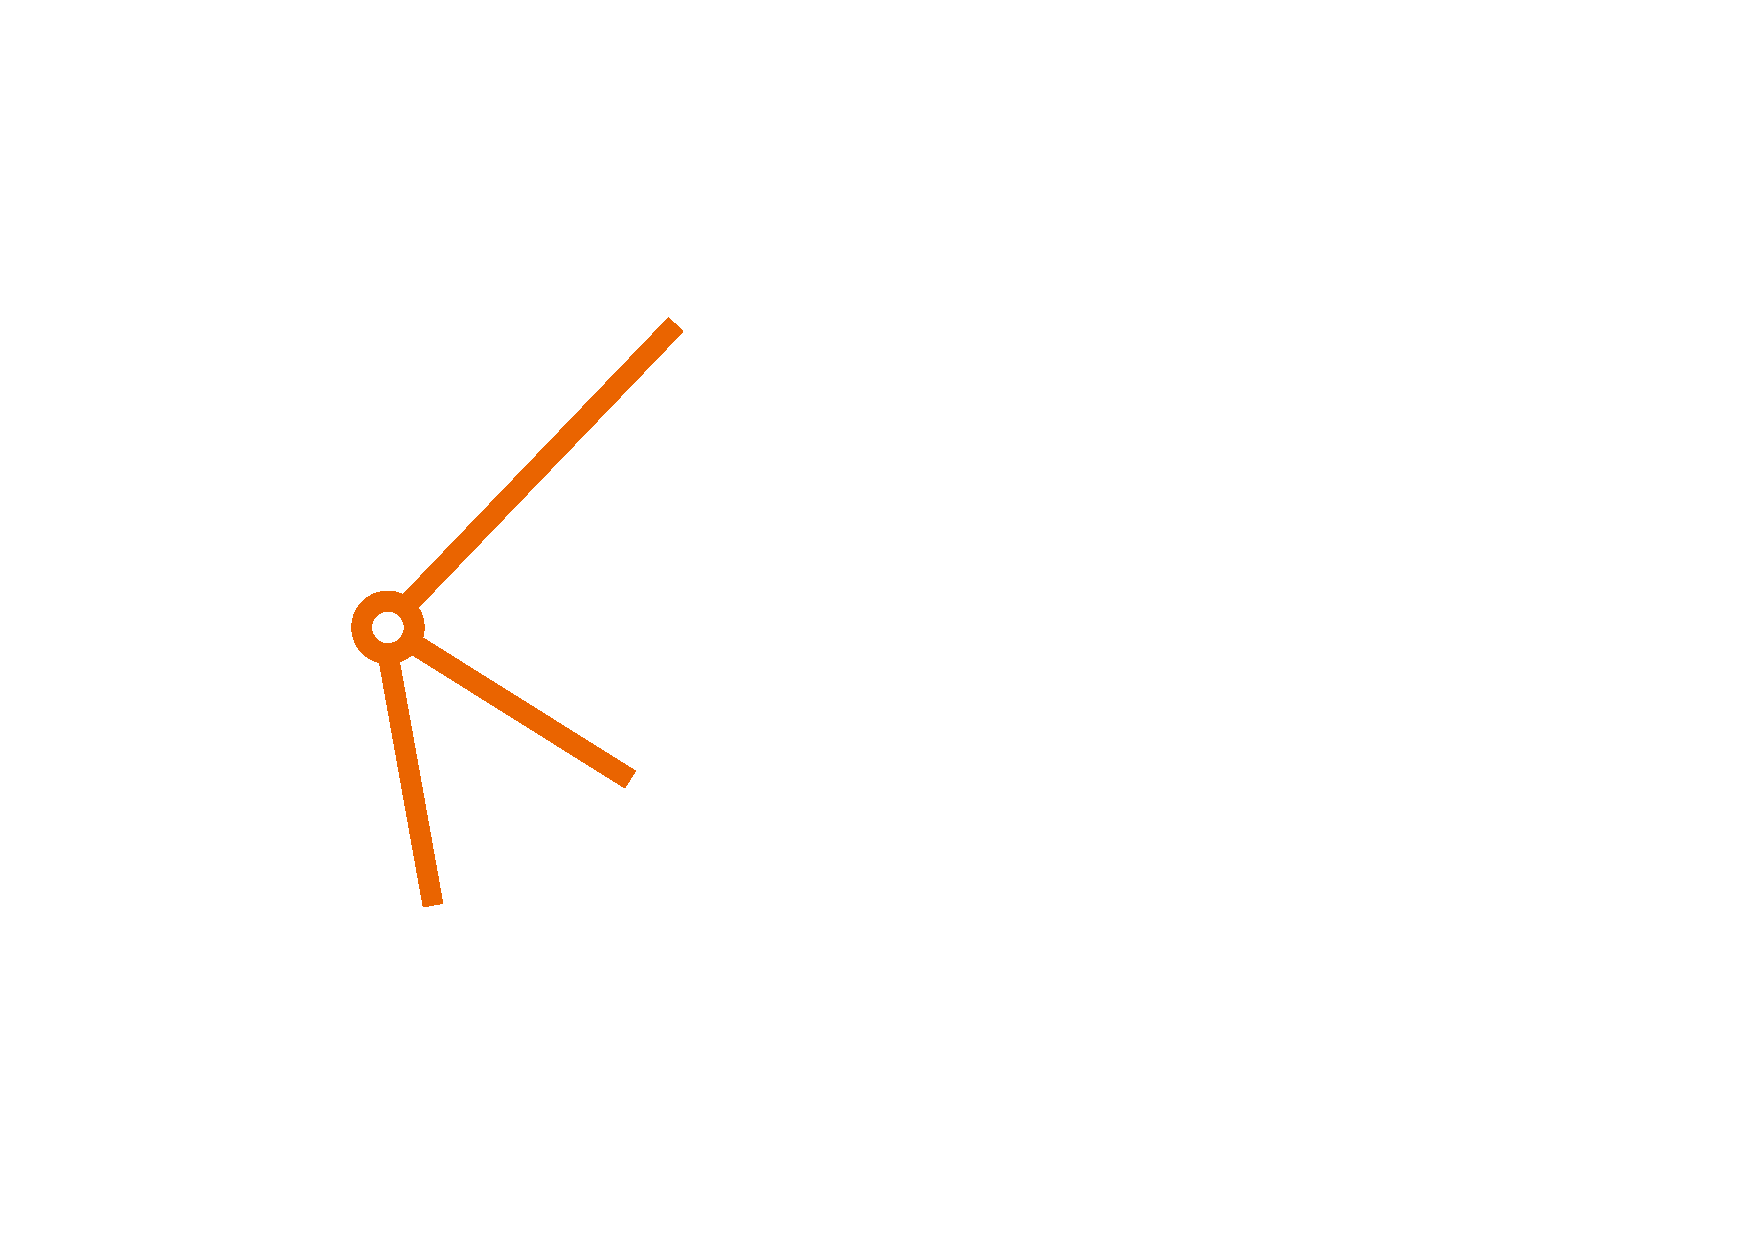
\includegraphics[scale=0.75]{line}};
\node[anchor=center,xshift=8cm,yshift=13cm]{
\includegraphics[scale=0.2]{ut_logo}};
\node[anchor=center,xshift=-10.0cm,yshift=11.8cm]{
\includegraphics[scale=0.5]{Pacman}};
\end{tikzpicture}

\begin{abstract}
In this work we implement Deep Q-Learning methods to solve the classic arcade game of Pacman. We compare two different models and the speed at which they learn to play the game on different size boards. We investigate the effect of using three different variants of experience replay and two different loss functions for a total of 36 independent experiments. We find that our model is able to learn faster than previous work and is even able to learn how to consistently win on the mediumClassic board after only 3,000 training episodes, previously thought to take much longer.
\end{abstract}

\begin{IEEEkeywords}
Deep Q-Learning, Priority Replay
\end{IEEEkeywords}

%--------------------------------------------------------------------------
\section{Introduction}
An important milestone in Reinforcement Learning (RL) research was a paper that showcased Deep Q-Learning models that could learn to play Atari games automatically \cite{Mnih2015}. Since then, many researchers have been interested in this field because video games offer controlled environments that many researchers can use to quickly iterate on their new RL algorithms. Then the algorithms they create can be applied to a wide variety of real world problems. So video games offer a great opportunity of having well defined environments with a great diversity of complexity.

In this work we use one of the most popular games of all time: Pacman. We use a popular Pacman environment implementation supplied by The University of California, Berkeley (UC Berkeley) \cite{berkeley_pacman}. We modified their environment to allow us to add our own agents, models, and replay memory. Figure \ref{fig:pacman-smallgrid} shows an example of one of the Pacman boards their environment provides.

\begin{figure}[h]
    \centering
    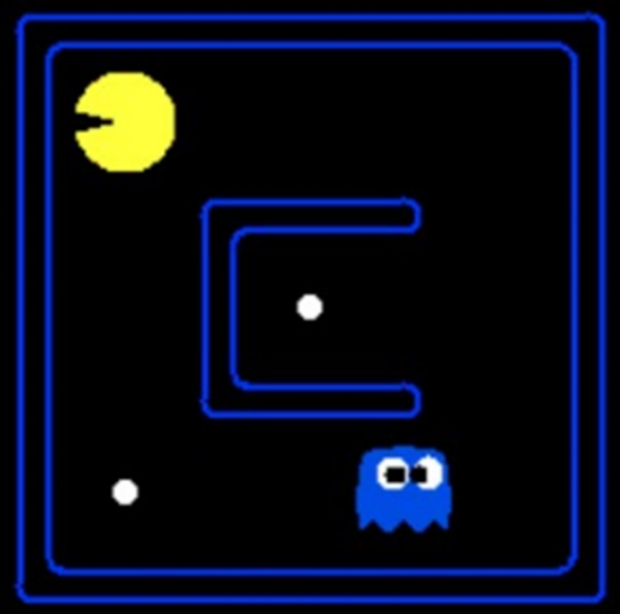
\includegraphics[scale=1.0]{pacman_small}
    \caption{A screenshot of the smallGrid environment.}
    \label{fig:pacman-smallgrid}
\end{figure}


%--------------------------------------------------------------------------
\section{Previous Work}
Relevant work related to Pacman was done by Mnih et al. \cite{MnihKSGAWR13} from DeepMind\footnote{https://deepmind.com}, where they present the first deep learning model as a function approximation. However, the experiments are applied to only few games and the ideas presented in the paper are no longer the standard for new RL research. For example, the authors use a semi-gradient method with a single neural network.

Another paper from DeepMind \cite{Mnih2015} was an important work to create a robust solution where they used memory replay and two networks in order to tackle the semi-gradient issue. They showed how their ideas are better at generalizing across a broad variety of Atari games. This work focuses on implementing the ideas from their paper such as memory replay and a Deep Q-Learning Network (DQN).

%\begin{figure*}[h]
%    \centering
%    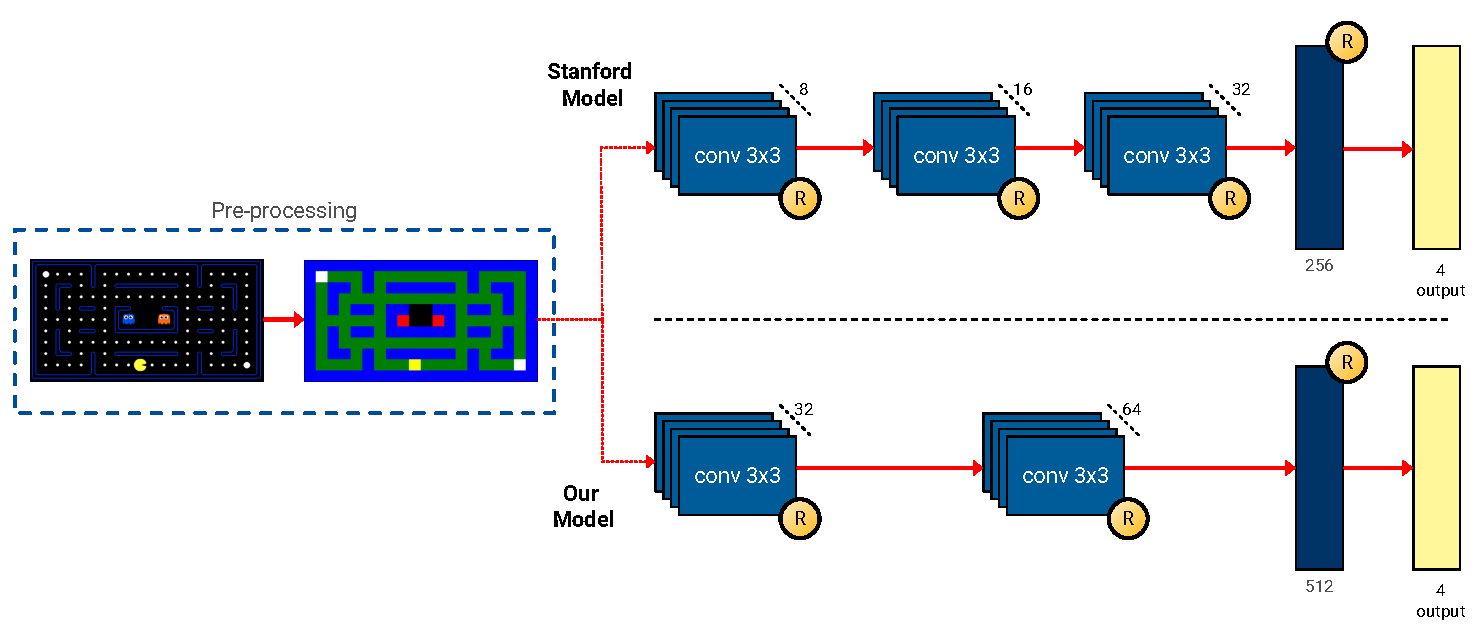
\includegraphics[scale=0.7]{models}
%    \caption{Illustration of the two models we used. On top: A proposed model by Gnanasekaran et al. \cite{stanford2017}. On bottom: Our proposed model}
%    \label{fig:models}
%\end{figure*}

\begin{figure*}
    \subfloat[]{\label{subfig:stanford}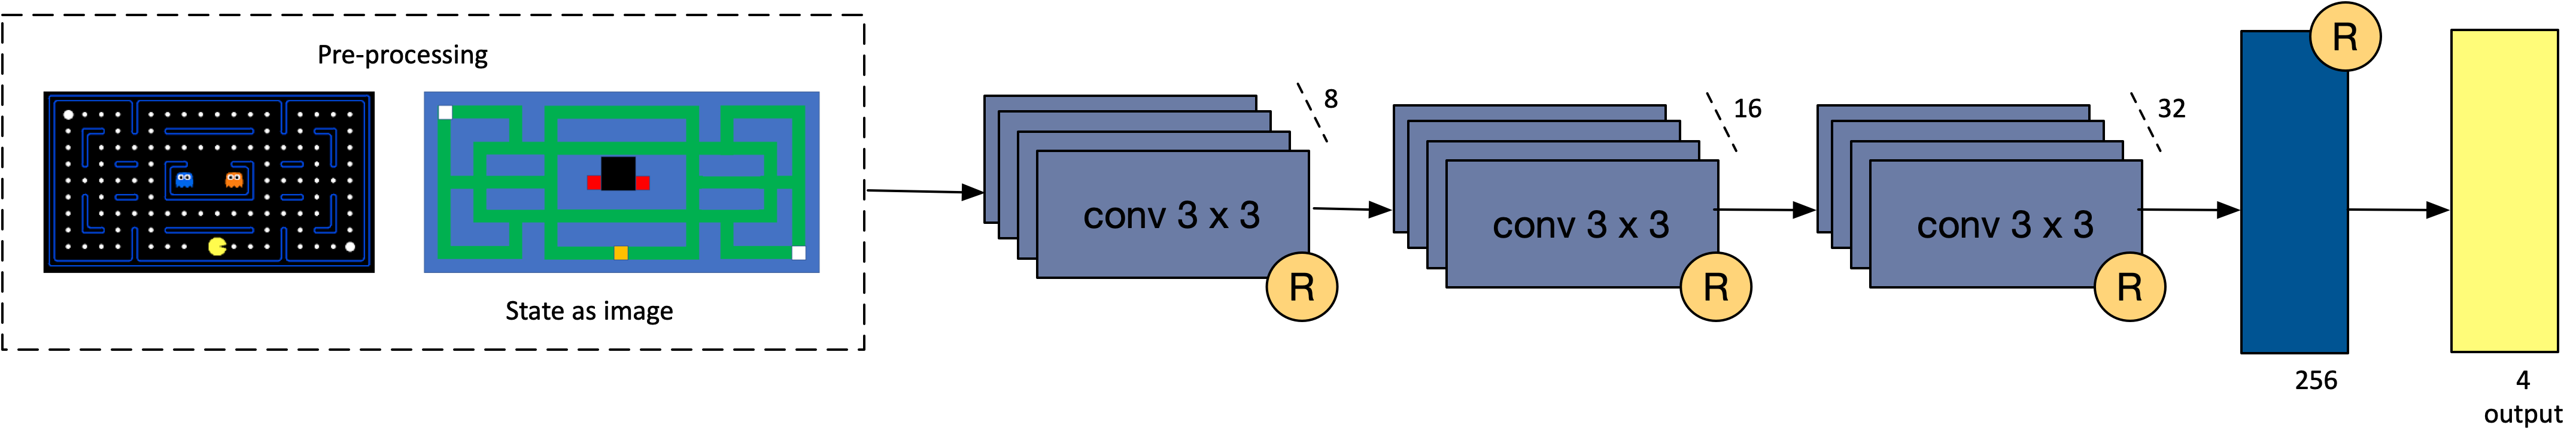
\includegraphics[width=\textwidth]{stateAsImageModel}} \\
    \subfloat[]{\label{subfig:ours}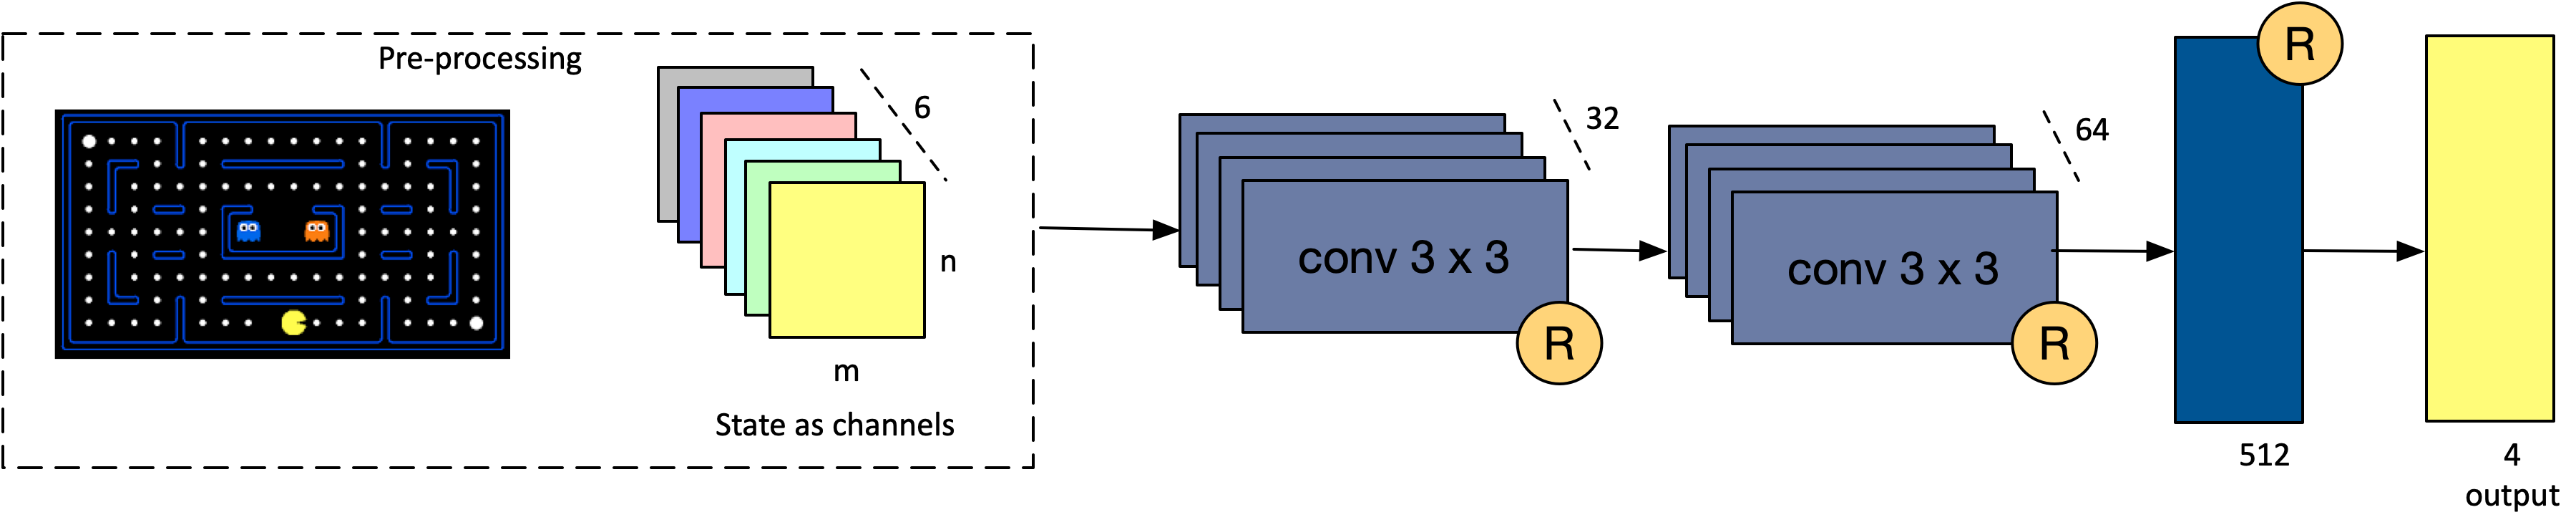
\includegraphics[width=\textwidth]{stateAsChannelsModel}}
    \caption{\ref{subfig:stanford} is the model proposed by Gnanasekaran et al. \cite{stanford2017} that preprocesses the state into an image and \ref{subfig:ours} is our model that converts the state into a 6 dimensional tensor}
    \label{fig:models}
\end{figure*}

It is important to indicate that this project is based on a popular template that is freely available and used as a project for a RL class \cite{berkeley_pacman}. We want to make note that there are many available repositories on the internet with various solutions to this problem. We chose to use PyTorch for two main reasons. The first is that many of those solutions are created using TensorFlow\footnote{https://github.com/advaypakhale/Berkeley-AI-Pacman-Projects}$^{,}$\footnote{https://github.com/jasonwu0731/AI-Pacman} and we do not want to be seen as replicating already established work. The second is because PyTorch is much more transparent in what each operation does and we find it is easier to understand from a glance as would a reader studying the implementation.

Dom{\'i}nguez-Est{\'e}vez et al. \cite{DomnguezEstvez2017TrainingPB} implemented a solution using DQN but they used the game ``Ms. Pacman vs. Ghosts'' from Gym\footnote{https://gym.openai.com} which is similar to the UC Berkeley environment but one provided by Gym does not offer any option to have a small environment as the one shown in Figure \ref{fig:pacman-smallgrid}.

Gnanasekaran et al. \cite{Abeynaya2017} show interesting results using memory replay, DQN, and Double DQN. We use some of their ideas in our work,  such as using the same model across different sized boards and implementing their model to test against ours.

In our work we added a few key improvements that we did not come across in any previous work. For example, all of the previous work used basic memory replay as suggested by Mnih et al. \cite{Mnih2015} but to the best of our knowledge no one has implemented prioritized replay when using Pacman with either of the open source available environments (Gym and UC Berkeley). We implemented prioritized replay memory using both variants presented by Schaul et al. \cite{schaul2016prioritized}, proportional and rank based.


%--------------------------------------------------------------------------
\section{Domain Problem} \label{sect:domain}

The problem we are working on is training an agent to play Pacman on different board sizes. The rules of Pacman are simple: eat all of the food and capsules while dodging the ghosts. The goal is then to do this as quickly as possible.

The state space of Pacman can be formulated as an MDP in multiple ways. There are six primary components that constitute the state of the game whose location needs to be kept track of.

\begin{itemize}
    \item Pacman: Where Pacman is currently at on the board.
    \item Ghost: Where the ghosts are currently at on the board.
    \item Capsules: The locations of the ``large'' dots. When Pacman eats a capsule, all of the ghosts become scared and edible.
    \item Food: The location of the ``small'' dots.
    \item Walls: The static positions of each wall on the board.
    \item Scared Ghosts: The location of ghosts that are scared and edible.
\end{itemize}

From these, we create two ways to concatenate the state so that the model can learn from it.

\paragraph{State as an image}
The first is by converting the Pacman board and state into an image ($n \times m \times 3$ tensor). We assign colors to each of the six different parts of the state, as done by \cite{stanford2017}.

\paragraph{State by channels}
The second is to create an $n \times m \times 6$ tensor where each channel corresponds to one of the different components of the state we care about. For instance, the first channel only contains the position of Pacman, while the second contains the location of walls, and so on.

As for the action space, like \cite{stanford2017} and \cite{berkeley_pacman}, we allow the cardinal directions and stopping to be valid actions. We use the rewards supplied by \cite{berkeley_pacman} as the rewards sent to our agent. To expand, the rewards were set with inspiration from the classic maze escape problem where the default is to give -1 point at all time steps, -500  if eaten by a ghost (losing), +10 for eating food, +200 for eating a scared ghost, and +500 for eating the last food capsule (winning).


%--------------------------------------------------------------------------
\section{Reinforcement Learning Methods}

Since our problem is fairly complicated, we think that using hand-crafted features and a large state, action array would be time-consuming and unfruitful. Instead we opted to explore Deep Q-Learning and its potential to solve complicated problems. Deep Q-Learning, introduced by \cite{Mnih2015}, suggests using two networks, a target and policy network, to perform Q-Learning using CNNs. We created two Deep Q-Learning networks with different goals in mind, to compare how well each is able to solve our problem. Figure \ref{fig:models} shows the two architectures we used in our experiments. The first one shown in Figure \ref{fig:models}a was suggested by Gnanasekaran et al. \cite{stanford2017} with three convolutional layers (8, 16, and 32 filters respectively) and a fully connected layer with 256 neurons. The second shown in Figure \ref{fig:models}b, was created by us with two convolutional layers (32 and 64 filters, respectively), and a fully connected layer with 512 neurons. We iterated towards this model by wanting to create simpler model in terms of feature extraction (hence two layers instead of three), and with more parameters to be able to learn the correct actions for more states. In both models, each layer is followed by a ReLU activation layer.

Because Deep Q-Learning relies on replaying past experiences to learn, we wanted to see if different types of replay functions could aid in solving the problem more quickly. Our base, a basic replay function, stores new experiences in a large deque that gets rid of old experiences once it starts to overfill, and when we perform training steps, it randomly samples 32 previous time-steps. There are two more methods of picking which previous time-steps to sample suggested by \cite{schaul2016prioritized} called Prioritized Experience Replay, and here we need to associate every experience with additional information (priority). The idea is to use the error of every sample and use that as the priority. In simple terms, the higher the error the higher the priority. So, first we take a sample batch from the memory replay and then we update the priority of this batch by using the error we got. Schaul et al. \cite{schaul2016prioritized} proposes two ways of getting priorities as follows:

\begin{itemize}
    \item Proportional: $p_i=|\delta_i|+\epsilon$, here the $\epsilon$ is a small value just to ensure that no sample will have zero probability, that way all the samples will have a chance to be picked
    \item Rank-based: $ p_i = 1/rank(i)$ sorts the priorities according to $|\delta| $ to get the rank
\end{itemize}

where $\delta$ is the error on that particular sample. It is also important to indicate that there are two hyper-parameters related to priority replay, $\alpha$ and $\beta$. As explained by Schaul et al. \cite{schaul2016prioritized}, $\alpha$ help us to determine the level of prioritization. So, we have that

\begin{equation}
    P(i)=\frac{p_{i}^{\alpha}}{\sum_{k}p_{i}^{\alpha}}
\end{equation}

The $\beta$ hyper-parameter is a weighting value that indicates how much we want to update the weights of the model. So, incorporating $\beta$ we have the formula:

\begin{equation}
    w_i = \left ( \frac{1}{N} \cdot \frac{1}{P(i))} \right )^\beta
\end{equation}

$\beta$ controls how much prioritization to apply to the current batch.

The suggested loss function for most reinforcement problems, to our knowledge, is Huber Loss. However, while we were initially creating these models and trying to get them to work, we noticed that sometimes using Mean Squared Error Loss would let the model converge more quickly. So for the purposes of our experiments, we run trials with both losses.

Overall, we have described a large number of parameters to tweak. One more parameter that we seek to analyze is the different board sizes supplied by our Pacman environment (smallGrid, mediumGrid, and mediumClassic, shown in Appendix \ref{appendix:grids}). In Table \ref{tab:experiments}, we summarize the options for each of these parameters. In total there are 36 experiments that we tested, one for each possible combination. We tested all three grid sizes provided by the UC Berkeley environment. We tested the Stanford model as defined in Gnanasekaran et al. \cite{stanford2017}, and our model (see figure \ref{fig:models}). To strictly follow the approach of Gnanasekaran et al. \cite{stanford2017}, we used images representing the states during training with their model while using a one-hot encoded binary structure for training with our model. Regarding the memory replay we test three approaches: basic memory replay as explained by Mnih et al. \cite{Mnih2015}, and proportional and rank-based prioritized memory replay as explained by Schaul et al. \cite{schaul2016prioritized}. And finally, we tried the two loss functions we previously described, MSE and Huber.

\begin{table}[]
\centering
\caption{The possible values for each of the four options we wanted to test the effect of. In total, there are 36 experiments (combinations, 3$\times$3$\times$2$\times$2) that we tested.}
\label{tab:experiments}
\begin{tabular}{c|c|c|c}
Grid Size & Model & Experience Replay & Loss Function \\ \hline
smallGrid & Stanford & Basic Replay & Mean Squared Error \\
mediumGrid & Ours & Proportional Priority & Huber Loss \\
mediumClassic &  & Rank-Based Priority &  \\
\end{tabular}
\end{table}



%--------------------------------------------------------------------------
\section{Code Design}

We used an object oriented design. We wrote everything outside of the \textit{pacman} folder except \textit{play.py}, which was supplied by UC Berkeley but heavily modified by us. \textit{agents.py} contains all code related agents playing the game.

Each Agent subclasses \textit{DQNAgent}, which provides all methods needed to play and train the models.
\begin{itemize}
  \item \textit{getAction}: Selects an action randomly or from the model, depending on the current $\epsilon$ value. Stores state-action data to the selected replay.
  \item \textit{epsilon}: Determines the current $\epsilon$ value for the $\epsilon$-greedy policy in \textit{getAction}
  \item \textit{final}: Called when an episode is finished to perform stat related calculations and set the weights of the target network to the ones of the policy network
  \item \textit{registerInitialState}: On the very first run, it calls \textit{build} to setup the initial models
  \item \textit{train\_step}: Performs a step of training. That entails: asking the replay for a batch of data, calculating the expected state action values, and performing one backpropagation step.
  \item \textit{build}: Implemented by subclass
  \item \textit{get\_state\_tensor}: Implemented by subclass
\end{itemize}

We have two agents that implement certain methods of \textit{DQNAgent}. The first is the one used with the Stanford model, \textit{ImageDQNAgent}.
\begin{itemize}
    \item \textit{build}: Creates a target and policy network using the Stanford model
    \item \textit{get\_state\_tensor}: Converts the state given by the UC Berkeley environment to an image like in \cite{stanford2017}
\end{itemize}
The second is our model, \textit{ChannelDQNAgent}.
\begin{itemize}
    \item \textit{build}: Creates a target and policy network using our model
    \item \textit{get\_state\_tensor}: Converts the state given by the UC Berkeley environment to a 6 channel tensor described in Section \ref{sect:domain}
\end{itemize}

We set up a script, \textit{experiments.py}, to run all of our experiments.

\textit{models.py} contains the PyTorch code for the Stanford and Our model.

Lastly we implement our replays in an object oriented manner as well. Each replay subclasses \textit{Replay}, which must provide a \textit{sample} method for getting a batch of timesteps, a \textit{push} method for saving new data, and \textit{weight\_losses} to allow priority replays to weight the losses.

%--------------------------------------------------------------------------
\section{Results Analysis}
As indicated in Table \ref{tab:experiments}, we ran 36 experiments where we combined the grid size (the size of the Pacman maze), the model (Stanford or our model), the three approaches for the memory replay (basic, prioritized-proportional, and prioritized-rank-based), and the loss function (Huber and MSE), and the results can be seen in figure \ref{fig:testing}.

\paragraph{Hyperparameters}
There are a number of hyperparameters that can be tweaked across runs that we needed to determine how to set. Our goal was to have results at least as good as the ones reported by Gnanasekaran et al. \cite{stanford2017} so we first started with the settings recommended in the paper. Unfortunately, using their settings with the models we had did not produce results that were optimal. Instead of 1500-2500 episodes needed for a 100\% win rate, we had to increase all of our models to 3,000 training episodes. The learning rate they suggested, $2.5\times 10^{-4}$ worked for that many training episodes. We also found that linearly decreasing $\epsilon$ from 1 to 0.1 as training went on worked well. We used these hyperparameter settings across all of our models for all of the grids. While we might be able to get better results using different hyperparameters in certain scenarios and parameter combinations, we wanted to give a fair comparison to all models across all of our parameter combinations so we kept them static across runs.

\begin{figure}
    \begin{subfigure}{.5\textwidth}
      \centering
      % include first image
      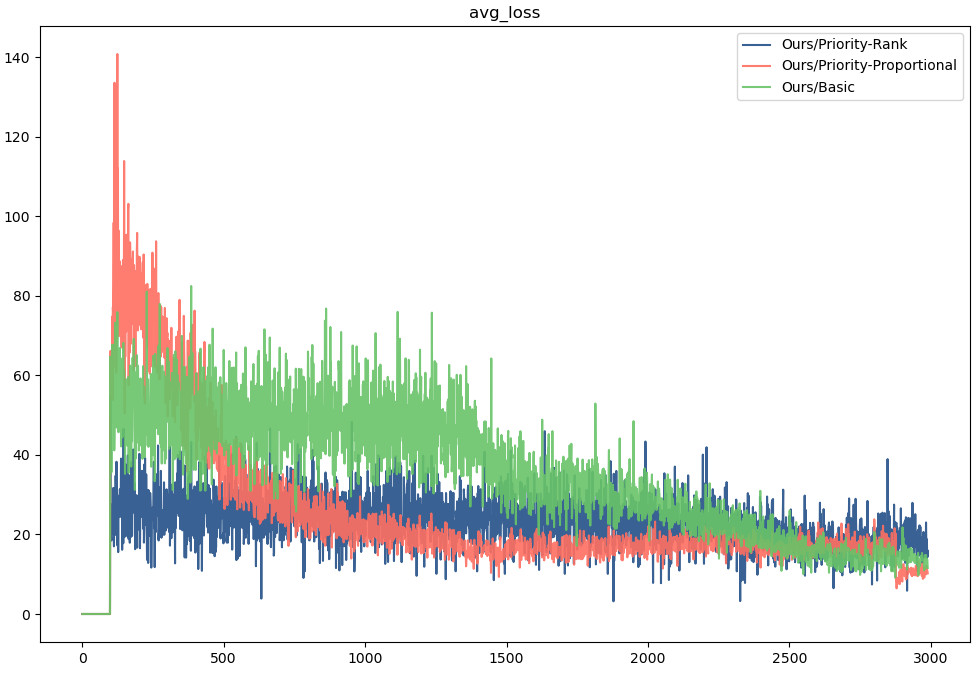
\includegraphics[width=.88\linewidth]{figures/small/training_smallgrid_huber_small.png}
      \caption{Huber loss and our model on the smallGrid layout.}
      \label{fig:train_our_huber}
    \end{subfigure}
    \begin{subfigure}{.5\textwidth}
      \centering
      % include second image
      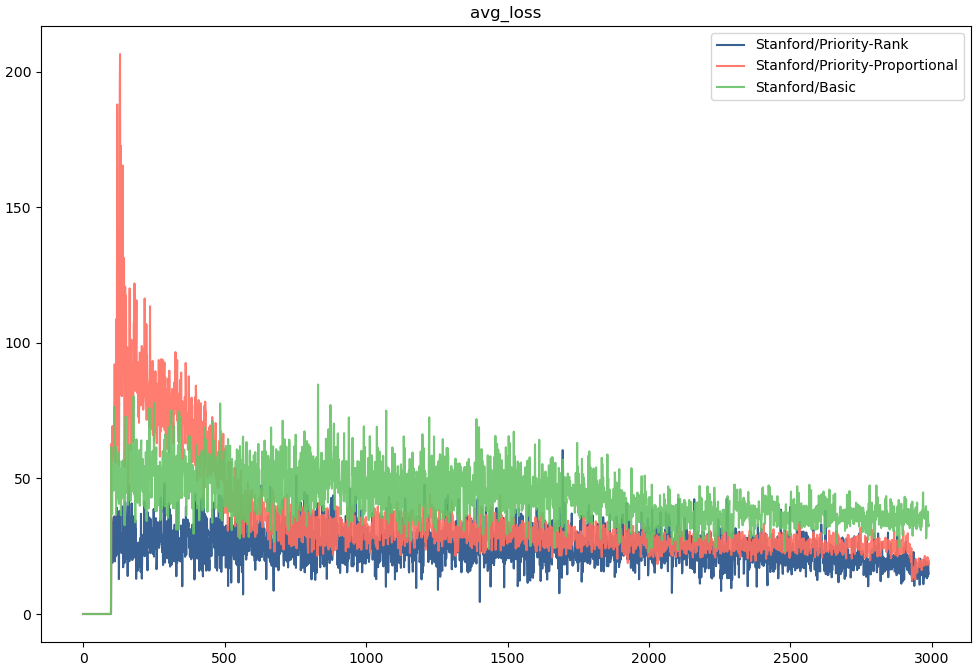
\includegraphics[width=.88\linewidth]{figures/small/training_smallgrid_huber_stanford.png}
      \caption{Huber loss and the Stanford model on the smallGrid layout.}
      \label{fig:train_stanford_huber}
    \end{subfigure}
    \newline

    \begin{subfigure}{.5\textwidth}
      \centering
      % include fourth image
      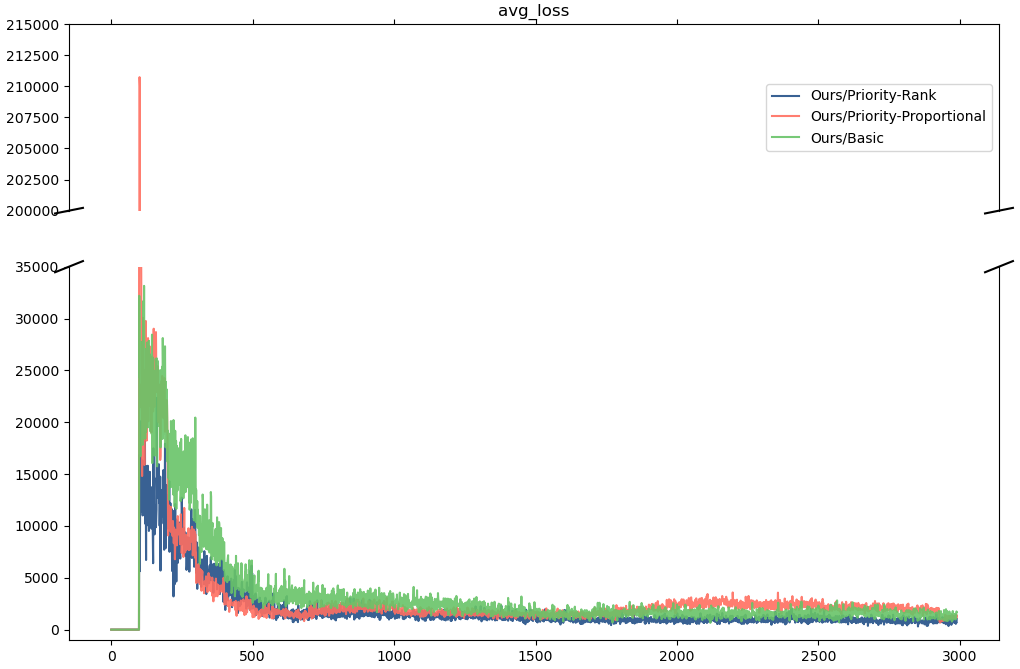
\includegraphics[width=.88\linewidth]{figures/small/training_smallgrid_mse_stanford.png}
      \caption{MSE loss and our model on the smallGrid layout.}
      \label{fig:train_our_mse}
    \end{subfigure}
    \begin{subfigure}{.5\textwidth}
      \centering
      % include third image
      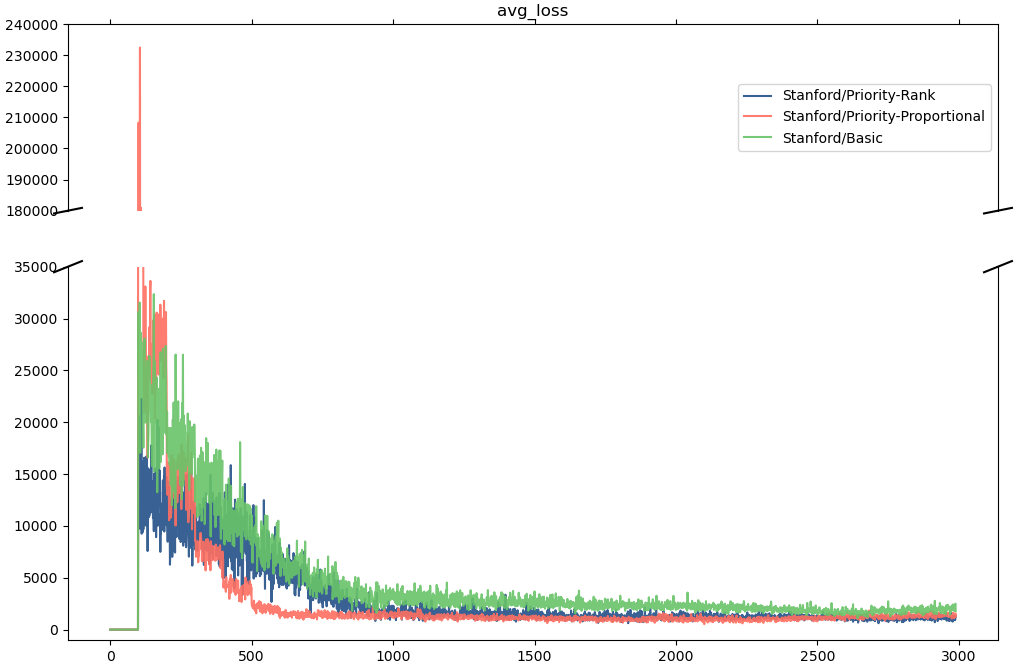
\includegraphics[width=.88\linewidth]{figures/small/training_smallgrid_mse_small.png}
      \caption{MSE loss and the Stanford model on the smallGrid layout.}
      \label{fig:train_stanford_mse}
    \end{subfigure}
    \caption{Loss plots during training with the three different approach of replay: basic, proportional, and rank-based.}
    \label{fig:training}
\end{figure}

\subsection{Loss Analysis and Training}

\begin{figure*}
    \centering
    \begin{subfigure}[b]{0.475\textwidth}
        \centering
        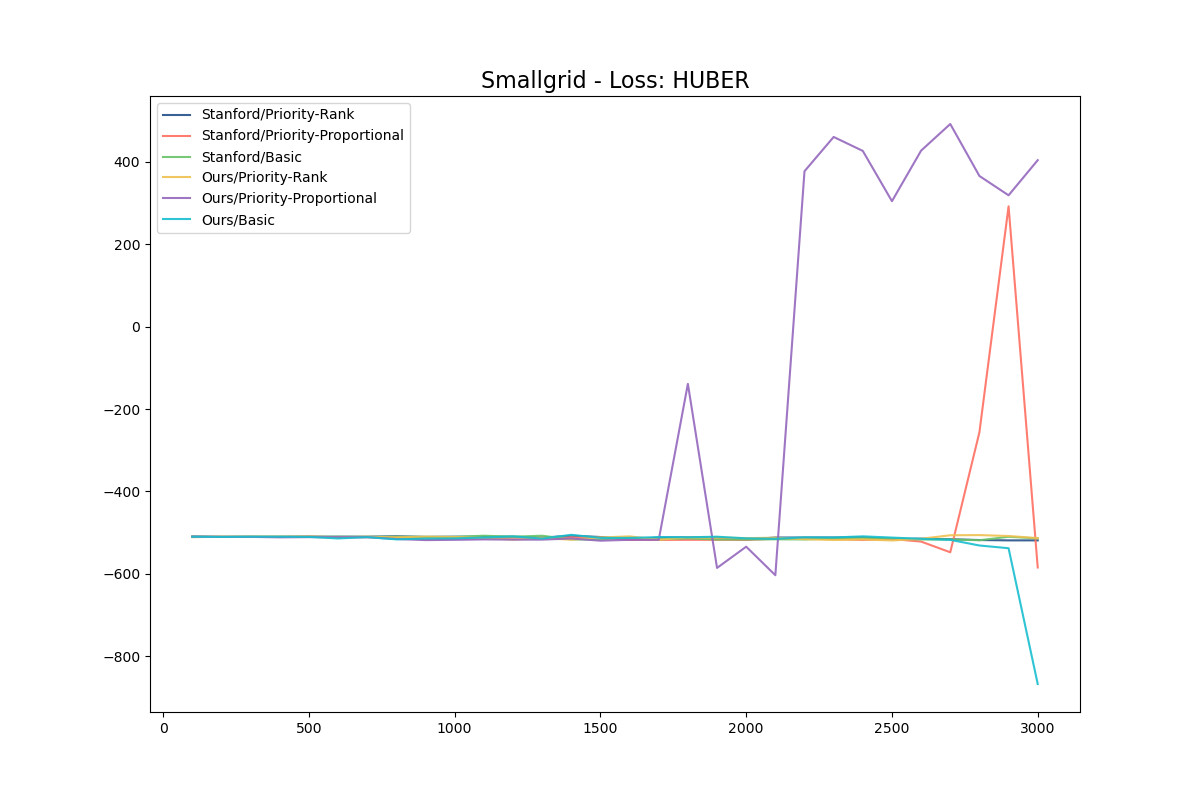
\includegraphics[width=\textwidth]{figures/small/testing_smallgrid_huber.png}
        \caption{smallGrid scores using Huber loss.}
        \label{fig:smallgrid_huber}
    \end{subfigure}
    \hfill
    \begin{subfigure}[b]{0.475\textwidth}
        \centering
        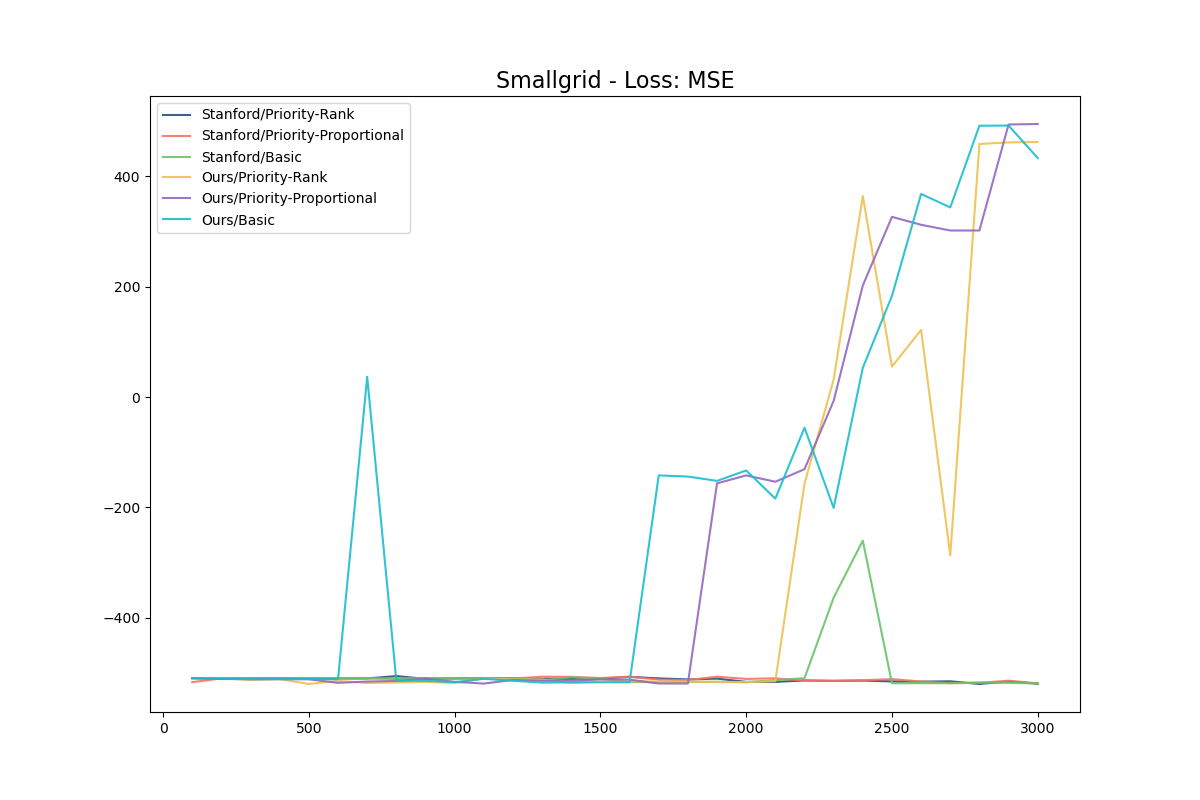
\includegraphics[width=\textwidth]{figures/small/testing_smallgrid_mse.png}
        \caption{smallGrid scores using MSE loss.}
        \label{fig:smallgrid_mse}
    \end{subfigure}
    \vskip\baselineskip
    \begin{subfigure}[b]{0.475\textwidth}
        \centering
        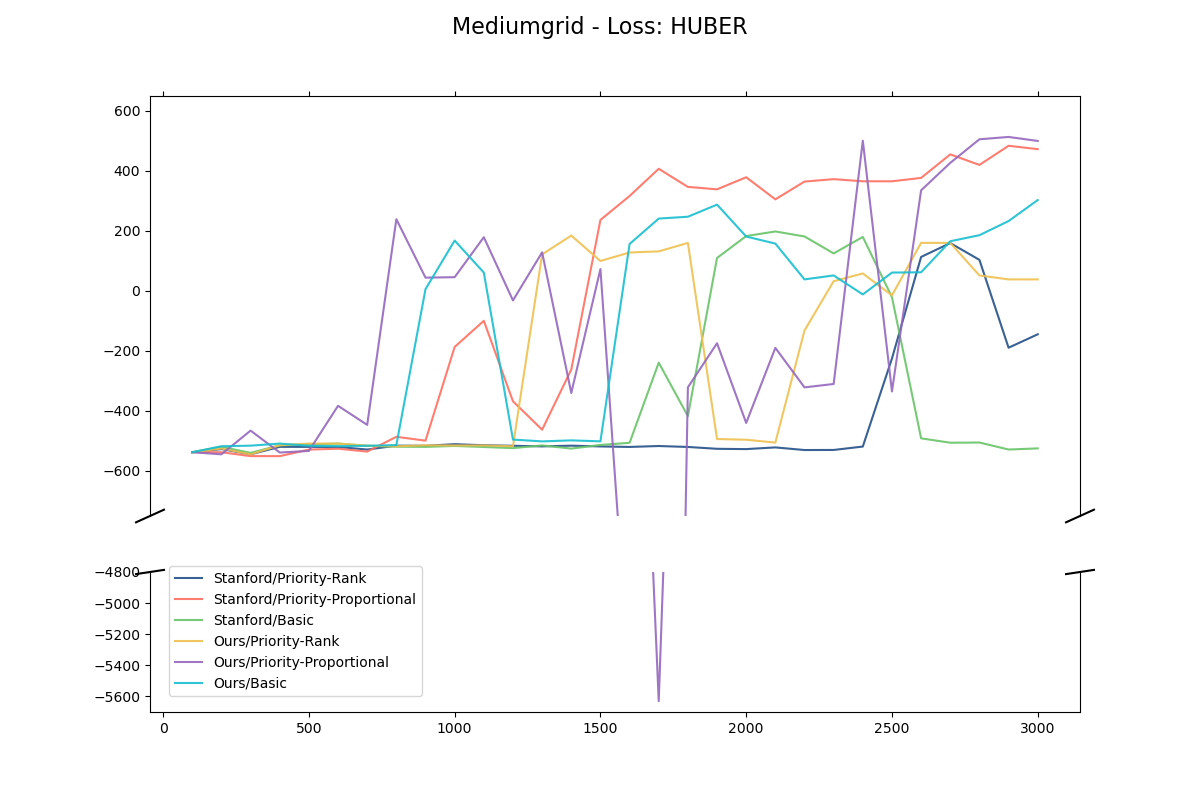
\includegraphics[width=\textwidth]{figures/medium/testing_mediumgrid_huber.png}
        \caption{mediumGrid scores using Huber loss.}
        \label{fig:mediumgrid_huber}
    \end{subfigure}
    \hfill
    \begin{subfigure}[b]{0.475\textwidth}
        \centering
        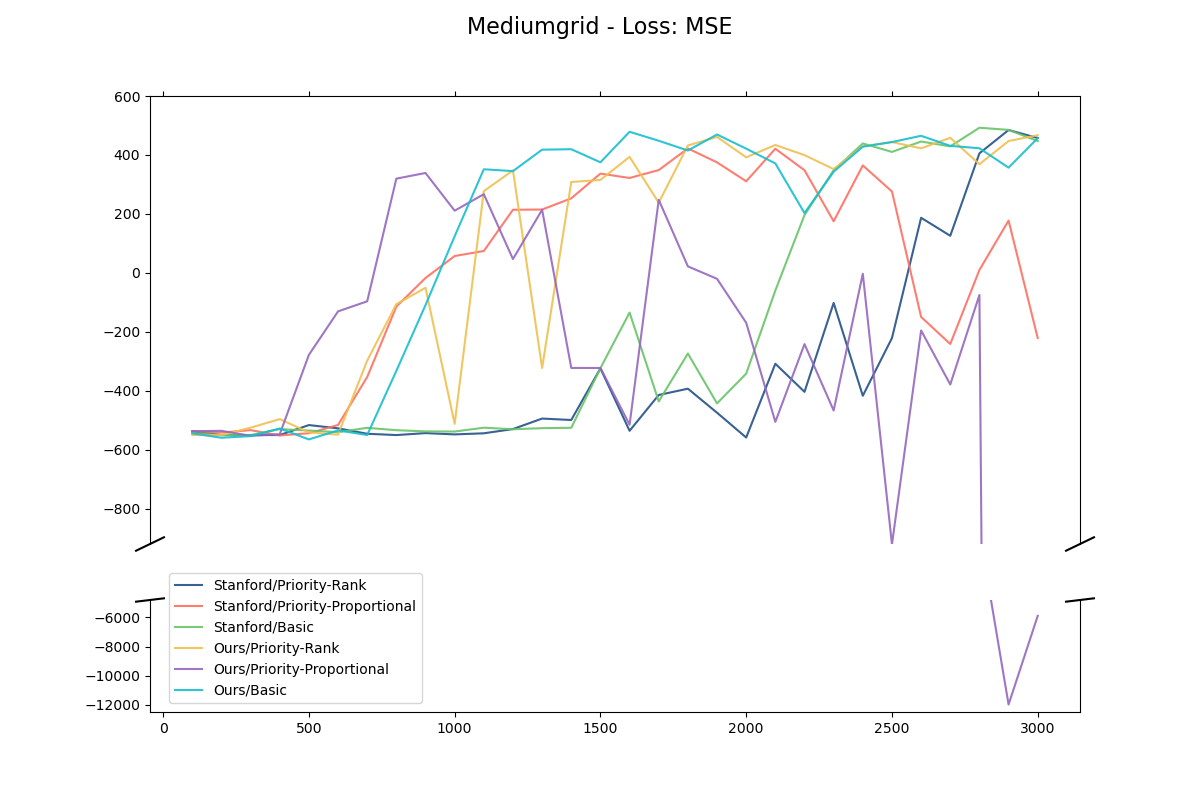
\includegraphics[width=\textwidth]{figures/medium/testing_mediumgrid_mse.png}
        \caption{mediumGrid scores using MSE loss.}
        \label{fig:mediumgrid_mse}
    \end{subfigure}
    \begin{subfigure}[b]{0.475\textwidth}
        \centering
        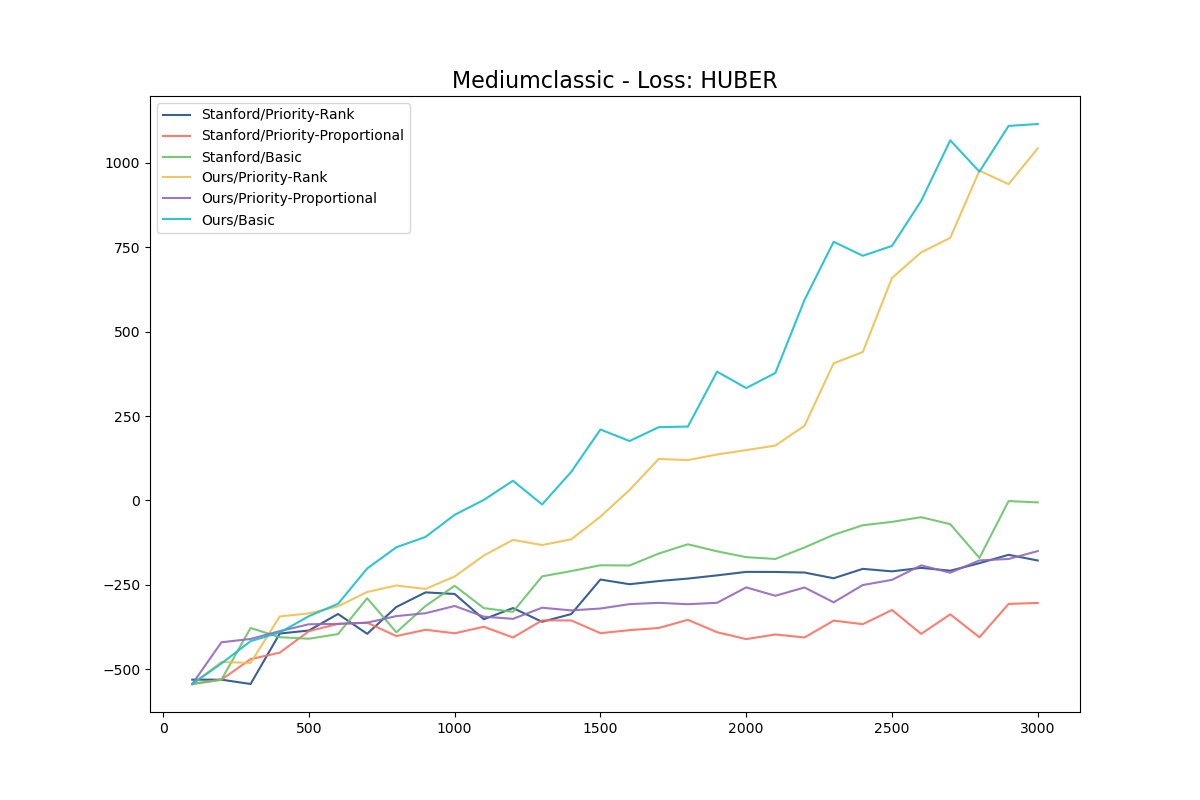
\includegraphics[width=\textwidth]{figures/mediumclassic/testing_mediumclassic_huber.png}
        \caption{mediumClassic grid scores using Huber loss.}
        \label{fig:mediumclassicgrid_huber}
    \end{subfigure}
    \hfill
    \begin{subfigure}[b]{0.475\textwidth}
        \centering
        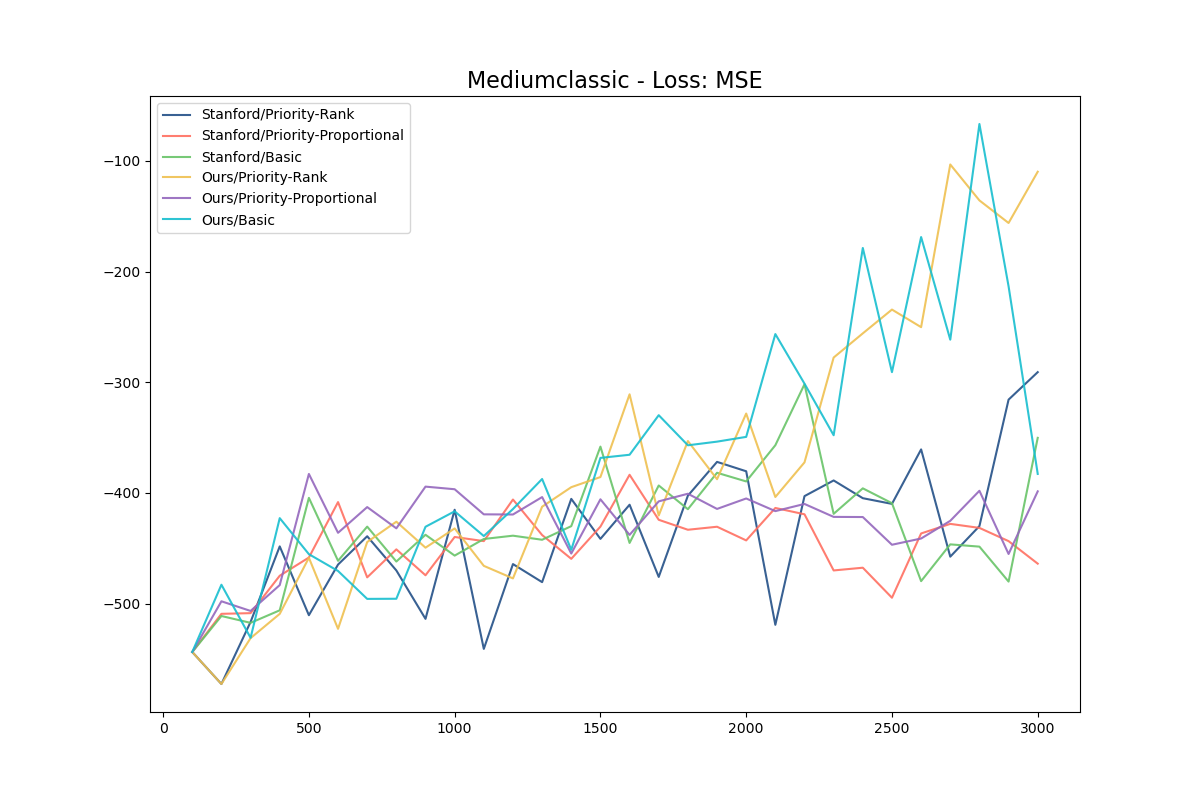
\includegraphics[width=\textwidth]{figures/mediumclassic/testing_mediumclassic_mse.png}
        \caption{mediumClassic grid scores using MSE loss.}
        \label{fig:mediumclassicgrid_mse}
    \end{subfigure}
    \vskip\baselineskip
    \caption{Results of the scores during testing. In every case we compared the three different memory replay approaches and the two models we used.}
    \label{fig:testing}
\end{figure*}

First, we want to discuss the behavior of the training related to our experiments. Figure \ref{fig:training} shows the results of the loss during training of the smallGrid by comparing the behavior of the three approaches we used for memory replay. Regarding the Huber loss, Figure \ref{fig:train_our_huber} shows that rank-based replay exhibits a slow convergence rate while basic and proportional replay have a more linearly decreasing behavior. In the intermediate episodes, proportional seems to converge faster and in the last episodes (2800-3000) proportional improves with an sudden fall to beat basic replay. Figure \ref{fig:train_stanford_huber} shows the case where basic replay has the worst behavior and rank-based has the best performance. An important aspect is to realize the size of the scale (the y-axis) between Figures \ref{fig:train_our_huber} and \ref{fig:train_stanford_huber}, where our model (Figure \ref{fig:train_our_huber}) has better results (smaller losses) during training.

Figures \ref{fig:train_our_mse} and \ref{fig:train_stanford_mse} show the behavior using MSE as the loss function. As seen, the three approaches of memory replay have a similar behavior, for example, it is hard to distinguish a real ``winner''in the last episode (3000), since the results are overlapping - as in the case of Figure \ref{fig:train_our_mse}, or pretty close to each other - as in the case of Figure \ref{fig:train_stanford_mse}. However, by looking at the small differences we can say that rank-based has the best performance since it shows a linearly decaying value in the average loss.


\subsection{Testing results}

Figure \ref{fig:testing} shows the testing results for all three grids using our model, the Stanford model, and the three versions of memory replay. Figure \ref{fig:smallgrid_huber} and \ref{fig:smallgrid_mse} show the results using the smallGrid. Interestingly, the smallGrid behaves better when using MSE during training, as seen in Figure \ref{fig:smallgrid_mse} where 3 out of 6 experiments show high/positive scores in the last episodes. However, using the Huber loss, just one model has an acceptable result (Figure \ref{fig:smallgrid_huber}). Also, the three successful experiments in Figure \ref{fig:smallgrid_mse} were using our model, and it can be seen that our proposed model surpasses the Stanford model in the smallGrid experiments using all three different replay memory approaches.

Figure \ref{fig:mediumgrid_huber} shows that in the case of using Huber loss, the Stanford model and ours have the best results when using prioritized proportional memory replay. Our model also has a good behavior when using the basic memory replay, and the rest of the combinations show erratic, unsuccessful behavior. In this case, it could be possible that more episodes would help to have more consistent and successful results. When using MSE (see Figure \ref{fig:mediumgrid_mse}) the behavior changes drastically where the Stanford and ours show the worst performance when using proportional replay. Furthermore, 4 out of 6 experiments have good results when using MSE, and it seems that the combination here of MSE and basic and rank-based replay have the best results, and our model (with basic replay and rank-based) is more consistent in converging.

Finally, we have the mediumClassic grid experiments in Figures \ref{fig:mediumclassicgrid_huber} and \ref{fig:mediumclassicgrid_mse}. The first one, using Huber, shows a trend to increase their scoring results. However, only our model using rank-based and basic replay is able to converge and consistently win on the mediumClassic board. That is not the case of Figure \ref{fig:mediumclassicgrid_mse}, where none of the models using MSE are able to converge. Of all the experiments we performed, this is the only ones where no positive scores were achieved.



%--------------------------------------------------------------------------
\section{Conclusions}

From the previous section we can say that MSE has better results in the smallGrid and mediumGrid with our initial setting of 3000 episodes. By using the smallGrid we found that only the proportional replay memory showed good results regardless of the loss function used. In the case of the mediumGrid, Huber loss performs better even though MSE also has good results. However, when using the mediumClassic grid which is the most complicated scenario, Huber has the best results over MSE which does not achieve any positive scoring. Consequently, with simple scenarios MSE is good enough and Huber is slow to converge, but for generalization purposes, Huber seems to be the right choice in the Pacman game, and most real Pacman levels are more similar to the mediumClassic experiment than to the smallGrid and mediumGrid ones.

Regarding the memory replay we found that in some cases the basic replay is good enough in some cases, this can be explained by the fact that the Pacman is not a complicated game -in terms of the goals to achieve- so, having the basic replay memory is an acceptable choice. The real advantages of rank-based and proportional memory replay are in specific scenarios, for example, proportional seems to be better in simple scenarios (smallGrid and mediumGrid) while rank-based seems to work better in more complex ones (mediumClassic). In any case, our model along with basic memory replay always shows promising results and it is the most consistent between all the different experiments.

Finally, we see throughout all the experiments that our proposed model performs better than the Stanford model. Our model has more filters and a larger dense layer, so, in this case having more weights equates to a better performance in Pacman.

%--------------------------------------------------------------------------
\section{Future Work}
We realize that choosing the model is extremely important in this problem, so an interesting path for future experimentation would be to apply a parameter search to find the best architecture for the model. Also, we found that using the one-hot encoding we got better results, having more challenging scenarios can give more confidence in order to generalize this finding. And finally, due to time constraints we did not implement double Deep Q-Networks (DDQN). It will be interesting to observe if DDQN can achieve comparable or better results that what we have achieved in the same or fewer episodes.

%--------------------------------------------------------------------------
\printbibliography[title={References}]

\appendix
\section{Grids} \label{appendix:grids}

In Figure \ref{fig:grids} we showcase what the different grids look like so the reader understands the complexity of each.

\begin{figure}
    \subfloat[]{\label{subfig:smallGrid}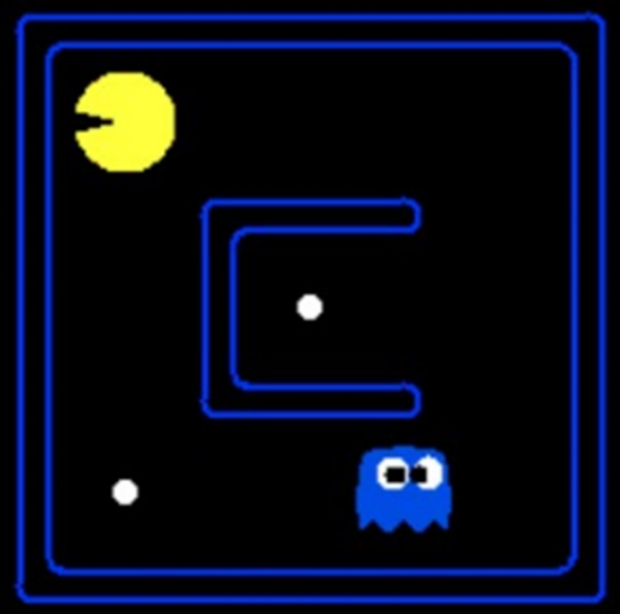
\includegraphics[width=0.3\textwidth]{pacman_small}} \\
    \subfloat[]{\label{subfig:mediumGrid}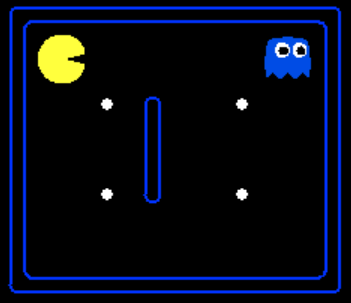
\includegraphics[width=0.35\textwidth]{mediumGrid}} \\
    \subfloat[]{\label{subfig:mediumClassic}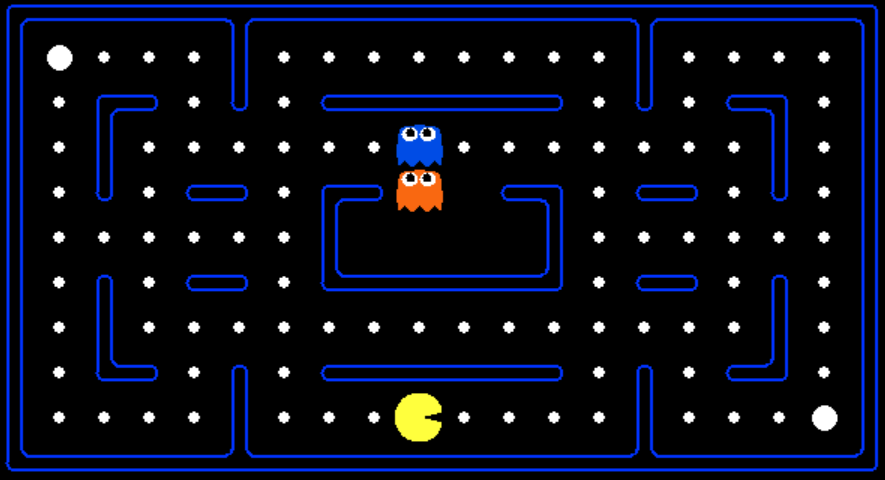
\includegraphics[width=0.5\textwidth]{mediumClassic}}
    \caption{All of the grid sizes that we test. \ref{subfig:smallGrid} is smallGrid, \ref{subfig:mediumGrid} is mediumGrid, and \ref{subfig:mediumClassic} is mediumClassic.}
    \label{fig:grids}
\end{figure}

\end{document}
